% --------------------------------------------------------------
% This is all preamble stuff that you don't have to worry about.
% Head down to where it says "Start here"
% --------------------------------------------------------------

\documentclass[12pt]{article}

\usepackage[margin=1in]{geometry}
\usepackage{amsmath,amsthm,amssymb}
\usepackage{pgf}
\usepackage{tikz}
\usetikzlibrary{arrows,automata}
\usepackage[latin1]{inputenc}
\usepackage{verbatim}

\newcommand{\N}{\mathbb{N}}
\newcommand{\Z}{\mathbb{Z}}

\newenvironment{theorem}[2][Theorem]{\begin{trivlist}
\item[\hskip \labelsep {\bfseries #1}\hskip \labelsep {\bfseries #2.}]}{\end{trivlist}}
\newenvironment{lemma}[2][Lemma]{\begin{trivlist}
\item[\hskip \labelsep {\bfseries #1}\hskip \labelsep {\bfseries #2.}]}{\end{trivlist}}
\newenvironment{exercise}[2][Exercise]{\begin{trivlist}
\item[\hskip \labelsep {\bfseries #1}\hskip \labelsep {\bfseries #2.}]}{\end{trivlist}}
\newenvironment{problem}[2][Problem]{\begin{trivlist}
\item[\hskip \labelsep {\bfseries #1}\hskip \labelsep {\bfseries #2.}]}{\end{trivlist}}
\newenvironment{question}[2][Question]{\begin{trivlist}
\item[\hskip \labelsep {\bfseries #1}\hskip \labelsep {\bfseries #2.}]}{\end{trivlist}}
\newenvironment{corollary}[2][Corollary]{\begin{trivlist}
\item[\hskip \labelsep {\bfseries #1}\hskip \labelsep {\bfseries #2.}]}{\end{trivlist}}

\begin{document}

% --------------------------------------------------------------
%                         Start here
% --------------------------------------------------------------

\title{Homework 1}%replace X with the appropriate number
\author{Erich Menge\\ %replace with your name
CSCI 4011 - Formal Languages and Automata Theory} %if necessary, replace with your course title

\maketitle

\begin{problem}{1}
Solve this problem with Induction \\
\subsection*{Basis Step}
\begin{align*}
{C_1} &= \frac{1}{4} \cdot ({(1)^4} + 2 \cdot {(1)^3} + {(1)^2}) = 1\\
{1^3} &= 1\surd
\end{align*}
\subsection*{Inductive Step}
\begin{align*}
{1^3} + {2^3} + ... + {k^3} + {(k + 1)^3} &= \frac{1}{4}({(k + 1)^4} + 2{(k + 1)^3} + {(k + 1)^2})\\
\frac{1}{4}{\rm{(}}{{\rm{k}}^4}{\rm{  +  2}}{{\rm{k}}^3}{\rm{  +  }}{{\rm{k}}^2}{\rm{)  +  (k  +  1}}{{\rm{)}}^3} &= \frac{1}{4}({(k + 1)^4} + 2{(k + 1)^3} + {(k + 1)^2})\\
& = \frac{1}{4}({k^4} + 4{k^3} + 6{k^2} + 4k + 1 + 2{k^3} + 6{k^2} + 6k + 2 + {k^2} + 2k + 1)\\
& = \frac{1}{4}({k^4} + 2{k^3} + {k^2}) + \frac{1}{4}(4{k^3} + 6{k^2} + 6{k^2} + 4k + 6k + 2k + 1 + 2 + 1)\\
& = \frac{1}{4}({k^4} + 2{k^3} + {k^2}) + \frac{1}{4}(4{k^3} + 12{k^2} + 12k + 4)\\
& = \frac{1}{4}({k^4} + 2{k^3} + {k^2}) + {k^3} + 3{k^2} + 3k + 1\\
& = \frac{1}{4}({k^4} + 2{k^3} + {k^2}) + {(k + 1)^3}
\end{align*}
\hfill Q.E.D
\end{problem} \newpage

\begin{problem}{2} Part c of Exercise 1.4 \\
\indent \(\{ w|\text{w has an even number of a's and one or two b's}\} \) \\

${A}$

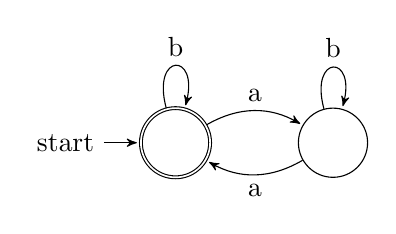
\begin{tikzpicture}[>=stealth',shorten >=1pt,auto,node distance=2cm]
  \node[initial,state,accepting] (S)      {};
  \node[state]         (q1) [right of=S]  {};
 \path[->]
 	(S)
 		edge [loop above] node{b}(S)
		edge [bend left]node{a}(q1)
	(q1)
		edge [loop above] node{b}(q1)
		edge [bend left]node{a}(S);

\end{tikzpicture} \\

${B}$ \\
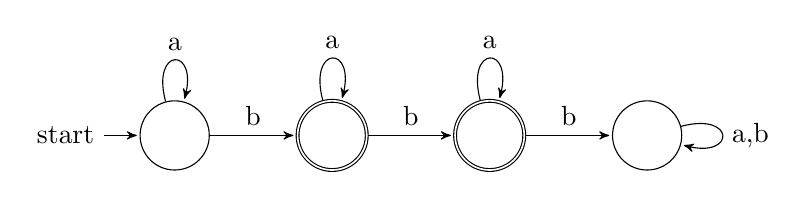
\begin{tikzpicture}[>=stealth',shorten >=1pt,auto,node distance=2cm]
  \node[initial,state] (S)      {};
  \node[state, accepting]         (q1) [right of=S]  {};
  \node[state, accepting]         (q2) [right of=q1]  {};
  \node[state]                    (q3) [right of=q2] {};
  \path[->]
    (S)
      edge [loop above] node{a}(S)
      edge              node{b}(q1)
    (q1)
      edge [loop above] node{a}(q1)
      edge node{b}(q2)
    (q2)
      edge [loop above] node{a}(q2)
      edge node{b}(q3)
    (q3)
      edge [loop right] node{a,b}(q3)
  ;
\end{tikzpicture} \\

${A \times B}$ \\
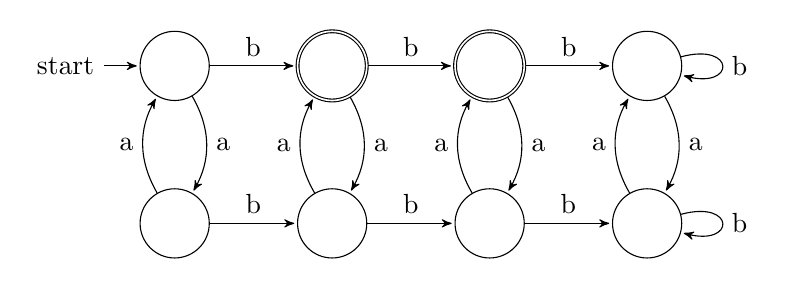
\begin{tikzpicture}[>=stealth',shorten >=1pt,auto,node distance=2cm]
  \node[initial, state] (a1b1) {};
  \node[state, accepting]  (a1b2) [right of=a1b1] {};
  \node[state, accepting]  (a1b3) [right of=a1b2] {};
  \node[state]          (a1b4) [right of=a1b3] {};

  \node[state] (a2b1) [below of=a1b1] {};
  \node[state] (a2b2) [right of=a2b1] {};
  \node[state] (a2b3) [right of=a2b2] {};
  \node[state] (a2b4) [right of=a2b3] {};

  \path[->]
    (a1b1)
      edge node{b}(a1b2)
      edge [bend left] node{a}(a2b1)
    (a1b2)
      edge node{b}(a1b3)
      edge [bend left] node{a}(a2b2)
    (a1b3)
      edge node{b}(a1b4)
      edge [bend left] node{a}(a2b3)
    (a1b4)
      edge [loop right] node{b}(a1b4)
      edge [bend left] node{a}(a2b4)

    (a2b1)
      edge node{b}(a2b2)
      edge [bend left] node{a}(a1b1)
    (a2b2)
      edge node{b}(a2b3)
      edge [bend left] node{a}(a1b2)
    (a2b3)
      edge node{b}(a2b4)
      edge [bend left] node{a}(a1b3)
    (a2b4)
      edge [loop right] node{b}(a2b4)
      edge [bend left] node{a}(a1b4)
  ;
\end{tikzpicture} \\
\end{problem}

\begin{problem}{3} Exercise 1.12 \\
\end{problem}

% --------------------------------------------------------------
%     You don't have to mess with anything below this line.
% --------------------------------------------------------------

\end{document}